\chapter{Graphical User Interfaces}
\label{chap:windows}

A \idx{command-line interface} (\idx{CLI}) is a method for communicating with the user through text. In contrast, a \idx{graphical user interface} (\idx{GUI}) also includes graphical elements such as  windows, icons, and sound, and a typical way to activate these elements are through a pointing device such as the mouse or by touch. Some of these elements may themselves be textual, and thus most operating systems offers access to a command-line interface in a window alongside other interface types.

Fsharp includes a number of implementations of graphical user interfaces, but at time of writing only \idx{WinForms} is supported on both the Microsoft .Net and the Mono platform, and hence, WinForms will be the subject of the following chapter.

WinForms is designed for \idx{event driven programming}, meaning that at run-time, most time is spend on waiting for the user to perform an action, called and \idx{event}, and each possible event has a predefined response to be performed. 

An example of a graphical user interface is a web-browser, as shown in Figure~\ref{fig:safariGui}.
\begin{figure}
  \centering
  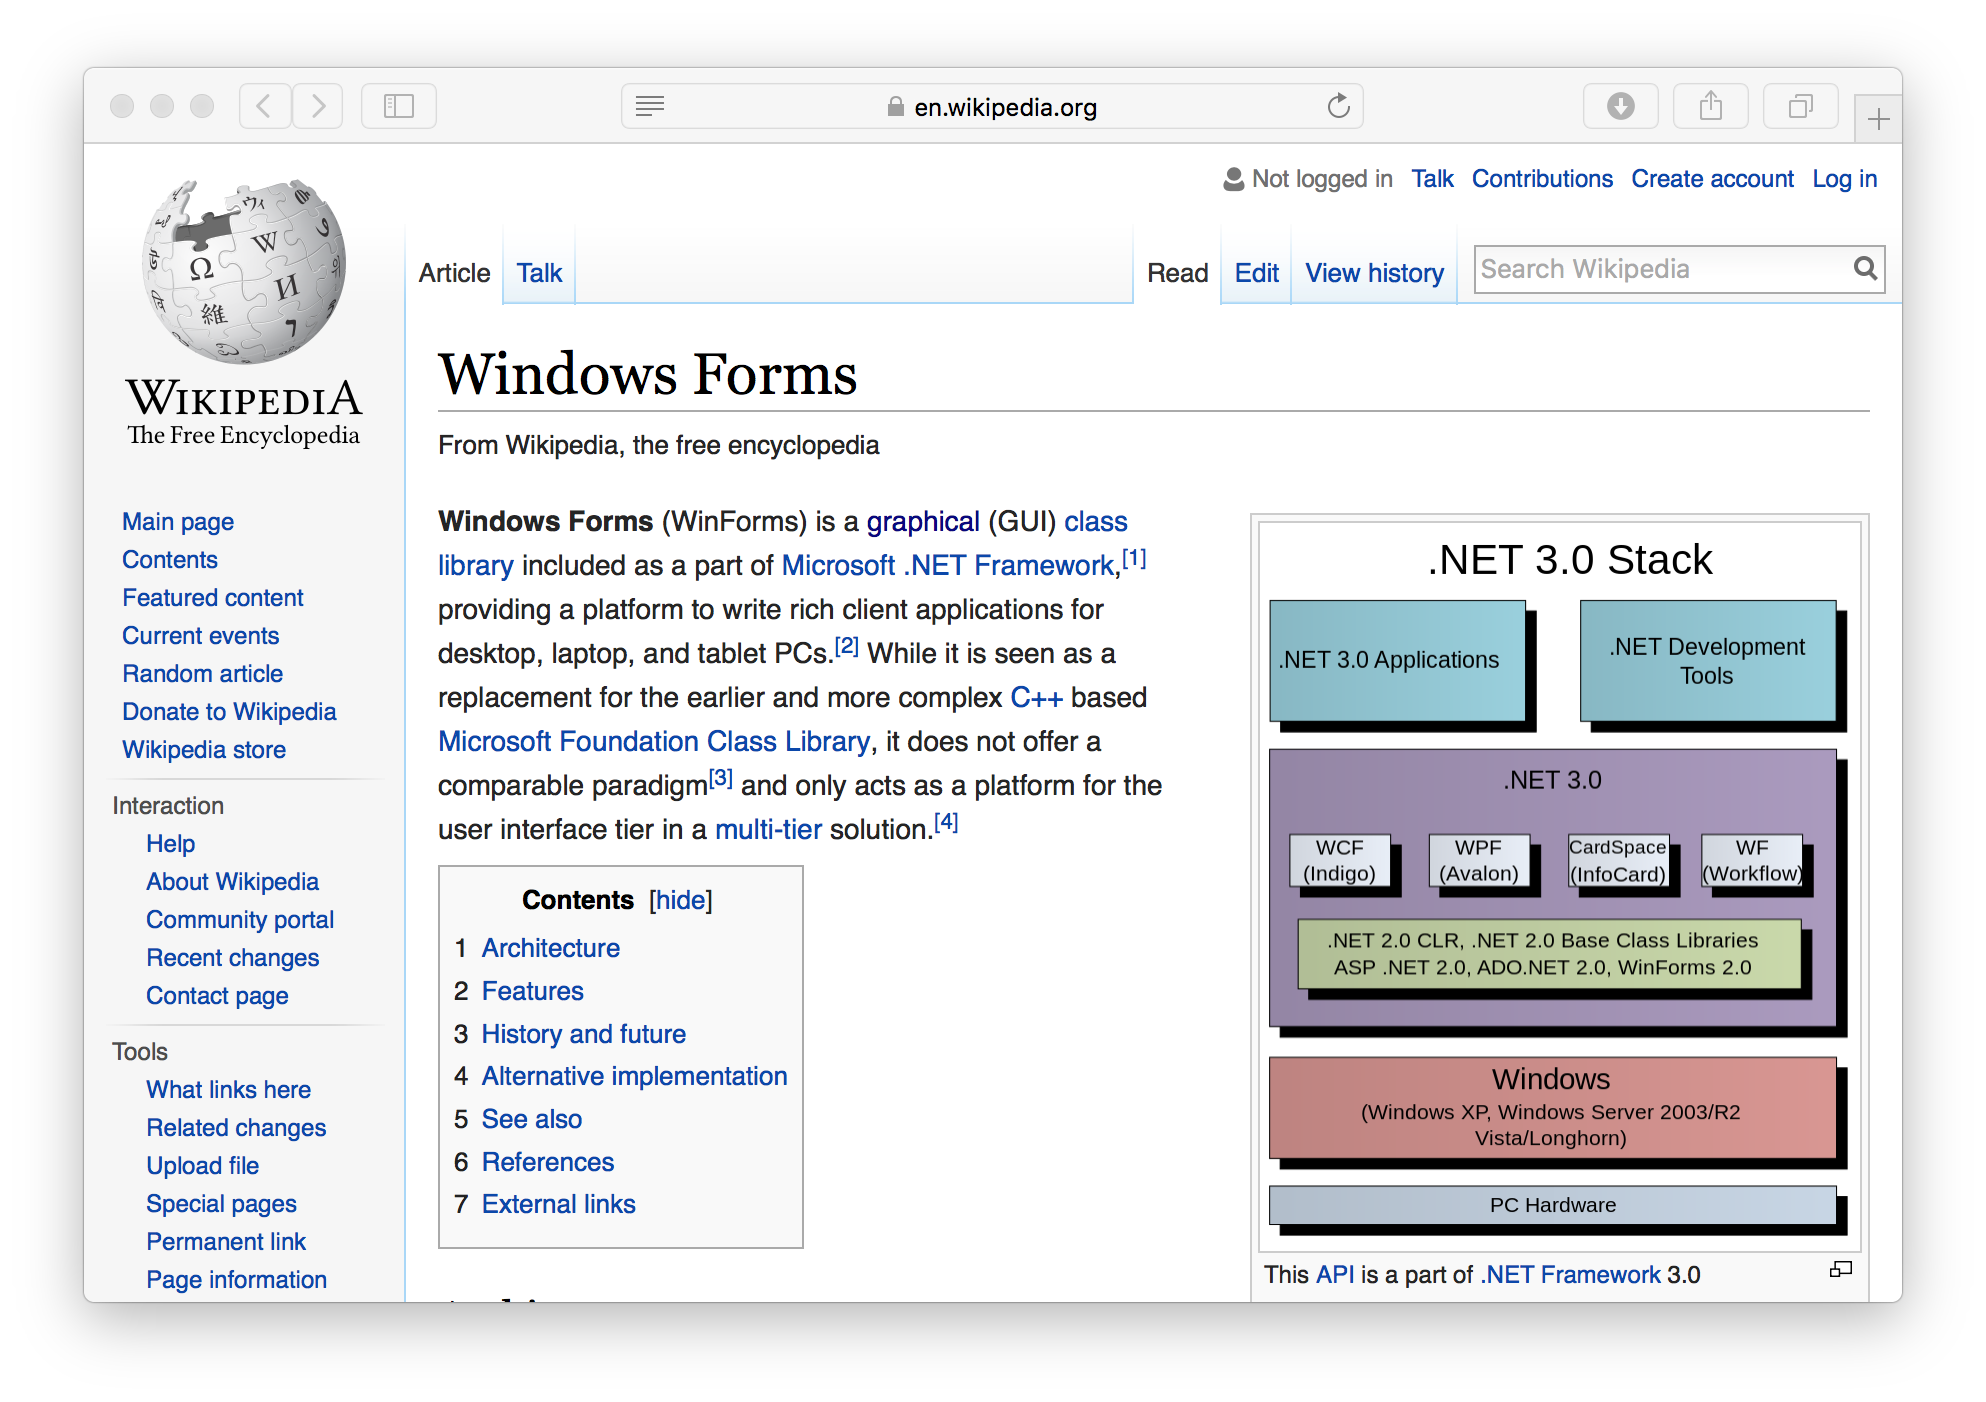
\includegraphics[width=0.8\textwidth]{safariWinForms}
  \caption{A web-browser is a graphical user interface for accessing a web-server and interacting with its services. Here the browser is showing the page \url{https://en.wikipedia.org/wiki/Windows_Forms} at time of writing.}
  \label{fig:safariGui}
\end{figure}
The program present information to the user in terms of text and images and has active areas that may be activated by clicking and which allows the user to go to other web-pages by type URL, to follow hyperlinks, and to generate new pages by entering search queries. Designing easy to use graphical user interfaces is a challenging task. This chapter will focus on examples of basic graphical elements and how to program these in WinForms.

\section{Drawing primitives in Windows}
The main workhorse of WinForms are the functions and classes defined in the namespaces: \idx{\lstinline{System.Windows.Forms}}  and \idx{\lstinline{System.Drawing}}. These give access to the \idx{Windows Graphics Device Interface} (\idx{GDI+}), which allows you to create and manipulate graphics objects targeting several platforms such as screens and paper. 

To display a graphical user interface on the screen, the first thing to do is open a window, which acts as a reserved screen-space for our output. In WinForms windows are called \idx{forms}. Code for opening a window is shown in Listing~\ref{winforms/openWindow}, and the result is shown in Figure~\ref{fig:openWindow}.
%
\fsCode{winforms/openWindow}{Create the window and turn over control to the operating system.}
%
\begin{figure}
  \centering
  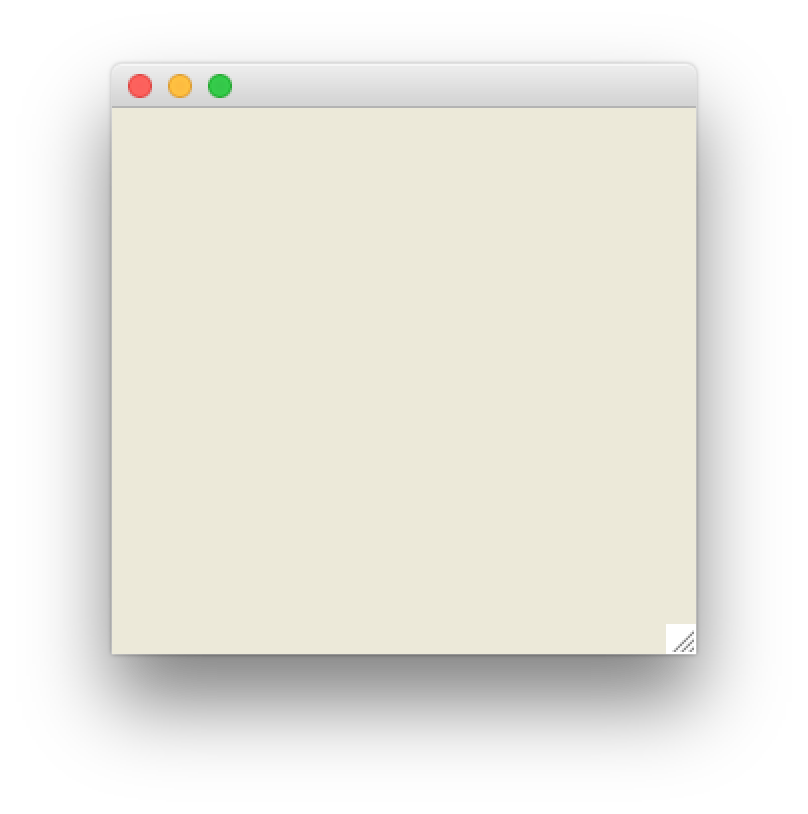
\includegraphics[width=0.6\textwidth]{openWindow}
  \caption{A window opened by Listing~\ref{winforms/openWindow}.}
  \label{fig:openWindow}
\end{figure}
The \lstinline!new System.Windows.Forms.Form ()! creates an object (See Chapter~\ref{chap:oop}), but does not display the window on the screen. When the function \lstinline!System.Windows.Forms.Application.Run! is applied to the object, then the control is handed over to the WinForms' \idx{event-loop}, which continues until the window is closed by, e.g., pressing the icon designated by the operating system. On the mac OSX that is the red button in the top left corner of the window frame, and on Window it is the cross on the top right corner of the window frame.

The window has a long list of \idx{methods} and \idx{properties}. E.g., the background color may be set by \lstinline!BackColor!, the title of the window may be set by \lstinline!Text!, and you may get and set the size of the window with the \lstinline!Size!. This is demonstrated in Listing~\ref{winforms/windowAttributes}.
%
\fsCode{winforms/windowAttributes}{Create the window and changing its properties.}
%
\begin{figure}
  \centering
  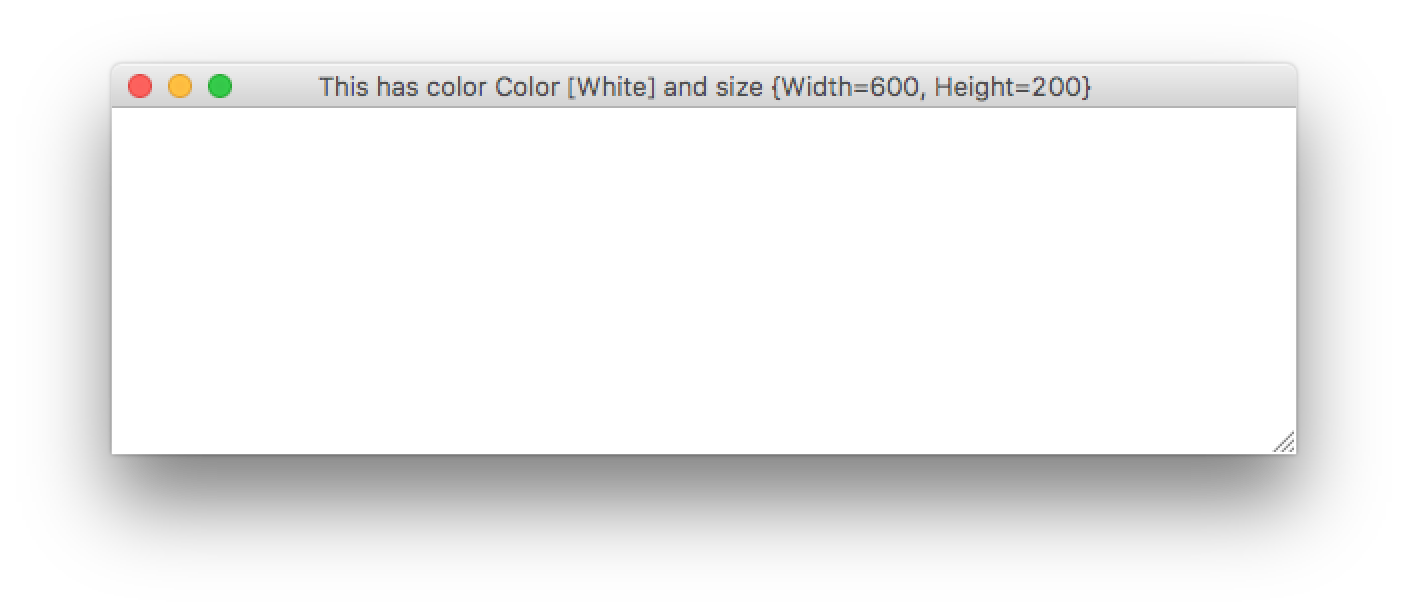
\includegraphics[width=0.6\textwidth]{windowAttributes}
  \caption{A window with user-specified size and background color, see Listing~\ref{winforms/windowAttributes}.}
  \label{fig:openWindow}
\end{figure}
These properties have been programmed as \idx{accessors} implying that they may used as mutable variables. 

The \idx{\lstinline{System.Drawing.Color}} is a general structure for specifying colors as 4 channels: alpha, red, green, blue. Some methods and properties for the Color structure is shown in Table~\ref{tab:color}.
\begin{table}
  \begin{center}
  \rowcolors{2}{oddRowColor}{evenRowColor}
    \begin{tabularx}{\linewidth}{|l|X|}
      \hline
      \rowcolor{headerRowColor}  Method/Property & Description\\
      \hline
      \lstinline{A}
      &Get the value of the alpha channel of a color.\\
      \hline
      \lstinline{B}
      &Get the value of the blue channel of a color.\\
      \hline
      \lstinline{Black}
      &Get a predefined color with ARGB value of \lstinline{0xFF000000}.\\
      \hline
      \lstinline{Blue}
      &Get a predefined color with ARGB value of \lstinline{0xFF0000FF}.\\
      \hline
      \begin{minipage}{0.45\linewidth}
        \lstinline{FromArgb : int -> Color}\\
        \lstinline{FromArgb : int*int*int*int -> Color}
      \end{minipage}
      &Create a color structure..\\
      \hline
      \lstinline{G}
      &Get the value of the green channel of a color.\\
      \hline
      \lstinline{Green}
      &Get a predefined color with ARGB value of \lstinline{0xFF00FF00}.\\
      \hline
      \lstinline{R}
      &Get the value of the red channel of a color.\\
      \hline
      \lstinline{Red}
      &Get a predefined color with ARGB value of \lstinline{0xFFFF0000}.\\
      \hline
      \lstinline{ToArgb : Color -> int}
      &Get the 32 bit integer representation of a color.\\
      \hline
      \lstinline{White}
      &Get a predefined color with ARGB value of \lstinline{0xFFFFFFFF}.\\
      \hline
    \end{tabularx}
  \end{center}
  \caption{Some methods and properties of the \lstinline{System.Drawing.Color}  structure.}
  \label{tab:color}
\end{table}
Each channel is an 8 bit unsigned integer, but often referred as the 32 bit unsigned integer by concatenating the channels. The alpha channel specifies the transparency of a color, where values 0--255 denotes the range of fully transparent to fully opaque, and the remaining channels denote the amount of red, green, and blue, where 0 is none and 255 is full intensity. Any color may be created using the \lstinline!FromArgb! method, e.g., an opaque red is given by \lstinline!System.Drawing.Color.FromArgb (255, 255, 0, 0)!. There are also many build-in colors, e.g., the same red color is also a known color and may be obtained as \lstinline!System.Drawing.Color.Red!. For a given color, then the 4 alpha, red, green, and blue channel's values may be obtained as the \lstinline!A!, \lstinline!R!, \lstinline!G!, \lstinline!B!, see Listing~\ref{drawingColors}
%
\fs{drawingColors}{Defining colors and accessing their values.}
%
The \lstinline!System.Drawing.Size! is a general structure for specifying sizes as height and width pair of integers. WinForms uses a number of types for specifying various objects some of which are shown in Table~\ref{tab:basicStructures}.
\begin{table}
  \begin{center}
  \rowcolors{2}{oddRowColor}{evenRowColor}
    \begin{tabularx}{\linewidth}{|l|X|}
      \hline
      \rowcolor{headerRowColor}  Constructor & Description\\
      \hline
      \begin{minipage}{0.4\linewidth}
        \lstinline{Point(int, int)}\\
        \lstinline{Point(Size)}
      \end{minipage}
      &An ordered pair of integers specifying x- and y-coordinates in the plane.\\
      \hline
      \begin{minipage}{0.4\linewidth}
        \lstinline{Size(int, int)}\\
        \lstinline{Size(Point)}
      \end{minipage}
      &An ordered pair of integers specifying height and width in the plane.\\
      \hline
     \begin{minipage}{0.4\linewidth}
       \lstinline{Rectangle(int, int, int, int)}\\
       \lstinline{Rectangle(Point, Size)}
     \end{minipage}
     &A structure specifying a rectangular region by its upper left corner and its size.\\
      \hline
    \end{tabularx}
  \end{center}
  \caption{Basic geometrical structures in WinForms.}
  \label{tab:basicStructures}
\end{table}
\jon{Note on difference between Size and ClientSize.}\jon{Do something about the vertical alignment of minpage.}

WinForms supports drawing of geometric primitives such as lines, rectangles, and ellipses, but not points. To draw an element similar to a point, you must draw a small rectangle or ellipse. The location and shape of geometrical primitives are specified in a coordinate system, and WinForms operates with 2 coordinate systems: \idx{screen coordinates} and \idx{client coordinates}. Screen coordinate $(x,y)$ have their origin in the top-left corner of the screen, and $x$ increases to the right, while $y$ increases down. Client coordinates refers to the drawable area of a form or a control, i.e., for a window this will be the area without the window borders, scroll and title bars. A control is a graphical object such as a clickable button, which will be discussed later. Conversion between client and screen coordinates is done with \idx{\lstinline{System.Drawing.PointToClient}} and \idx{\lstinline{System.Drawing.PointToScreen}}. To draw geometric primitives, we must also specify the pen using
for line like primitives and the brush for filled regions.

Displaying graphics in WinForms is performed as the reaction to an event. E.g., windows are created by the program, moved, minimized, occluded by other windows, resized, etc., by the user or the program, and each action may require that the content of the window is refreshed. Thus, we must create a function that WinForms can call any time. This is known as a \idx{call-back function}, and it is added to an existing form using the \idx{\lstinline{Paint.Add}} method. Due to the event-driven nature of WinForms, functions for drawing graphics primitives are only available when responding to an event, e.g., \idx{\lstinline{System.Drawing.Graphics.DrawLines}} draws a line in a window, and it is only possible to call this function, as part of an event handling.

As an example, consider the problem of drawing a triangle in a window. For this we need to make a function that can draw a triangle not once, but any time. An example of such a program is shown in Listing~\ref{winforms/triangle}.
%
\fsCode{winforms/triangle}{Adding line graphics to a window.}
%
\begin{figure}
  \centering
  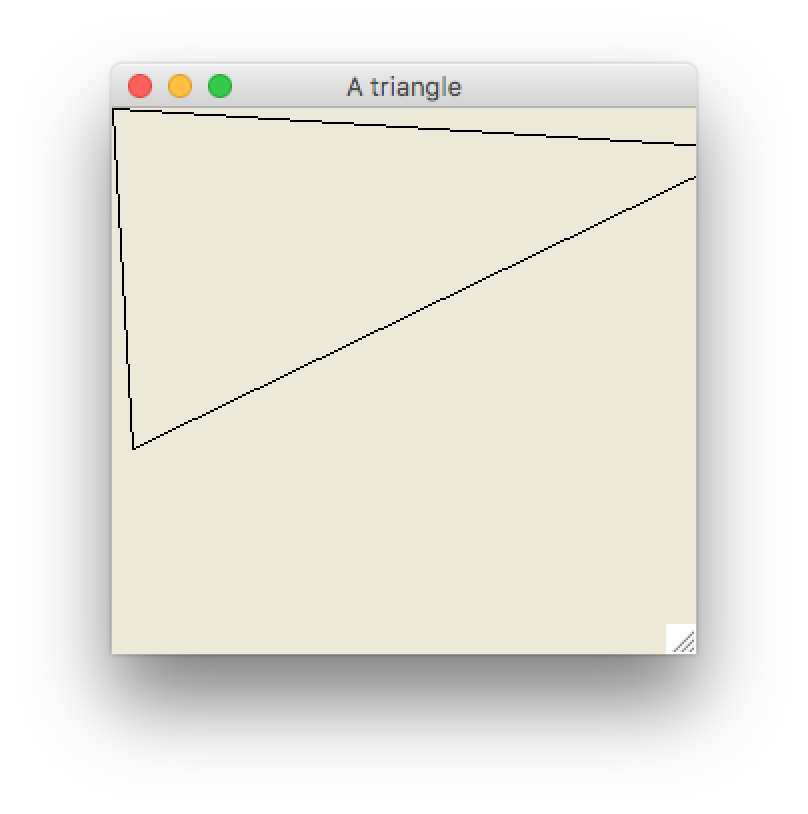
\includegraphics[width=0.6\textwidth]{triangle}
  \caption{Drawing a triangle using Listing~\ref{winforms/triangle}.}
  \label{fig:triangle}
\end{figure}
A walk-through of the code is as follows: First we create an array of points and a pen color, then we create a pen and a window. The method for drawing the triangle is added as an anonymous function using the created window's \lstinline!Paint.Add! method. This function is to be called as a response to a paint event and takes a \lstinline!System.Windows.Forms.PaintEventArgs! object, which includes the System.Drawing.Graphics object. Since this object will be related to a specific device, when the window's \lstinline!Paint! method is called, then we may call the \lstinline!System.Drawing.Graphics.DrawLines! function to sequentially draw lines between our array of points. Finally, we hand the form to the event-loop, which as one of the earliest events will open the window and call the \lstinline!Paint! function we have associated with the form.

Considering the program in Listing~\ref{winforms/triangle}, we may identify a part that concerns the specification of the triangle, or more generally the graphical model, some parts which handling events, and some which concerns system specific details on initialization of the interface. For future maintenance, it is often a good idea to \advice{separate the model from the implementation}. E.g., it may be that at some point, you decide that you would rather use a different library than WinForms. In this case, the general graphical model will be the same but the specific details on initialization and event handling will be different. While it is not easy to completely separate the general from the specific, it is often a good idea to strive some degree of separation. E.g., in Listing~\ref{winforms/triangle}, the program has been redesigned to make use of an initialization function and a paint function.
%
\fsCode{winforms/triangleOrganized}{Improved organization of code for
  drawing a triangle. Compare with Listing~\ref{winforms/triangle}.}
%
\begin{figure}
  \centering
  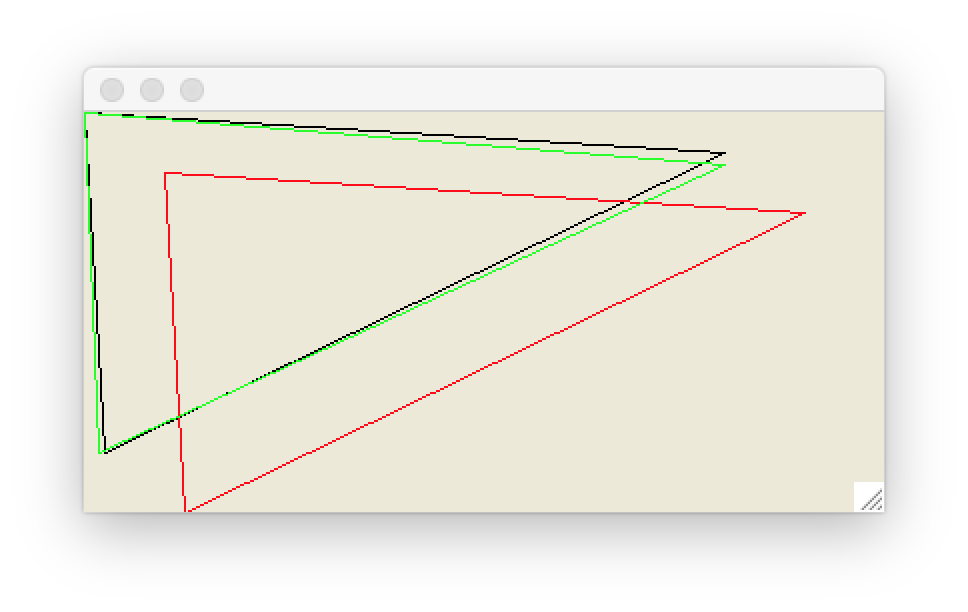
\includegraphics[width=0.6\textwidth]{triangleOrganized}
  \caption{Better organization of the code for drawing a triangle, see Listing~\ref{winforms/triangleOrganized}.}
  \label{fig:triangleOrganized}
\end{figure}
While this program is longer, to this author there is a much better separation of {\em what} is to be displayed from the {\em how} it is to be done, since the {\em how} is not contained in the functions \lstinline!createForm! and \lstinline!drawPoints!. The user-defined types \lstinline!coordinates! and \lstinline!pen! further emphasizes the semantic content of the data structures in use and makes use of Fsharp's type checker to reduce run-time errors.
\jon{requires the introduction of type declarations.}\jon{Remember to talk about pen width.}

Organizing code into functions that operate on data structures as Listing~\ref{winforms/triangleOrganized} is the first step in \idx{Structured programming} to be discussed in Part~\ref{part:structured}. Consider the case, where are to draw two new triangles, that are a translation and a rotations of the original. A simple extension of Listing~\ref{winforms/triangleOrganized} is to make a list of lists of Points and to extend \lstinline!drawPoints! with a loop for drawing all shapes in the list. This structure should include the ability to draw shapes in different styles, hence we arrive at a structure of type \lstinline!(coordinates * pen) list!. Furthermore, since the problem is to draw the same shape at different locations and orientations, instead of calculating the new coordinates by hand, it is useful to add functions to translate and rotation a given shape. Thus we arrive at the program shown in Listing~\ref{winforms/transformWindows}, and which results in the output shown in
Figure~ \ref{fig:transformWindow}.
%
\fsCode[numbers=left,numbersep=6pt,numberstyle=\scriptsize\color{white},lastline=42]{winforms/transformWindows}{Reusable  code for drawing in windows.}
\fsCode[numbers=left,numbersep=6pt,numberstyle=\scriptsize\color{white},firstnumber=44,firstline=44]{winforms/transformWindows}{Code for drawing triangles using the reusable part shown in Listing~\ref{winforms/transformWindows}.}
%
\begin{figure}
  \centering
  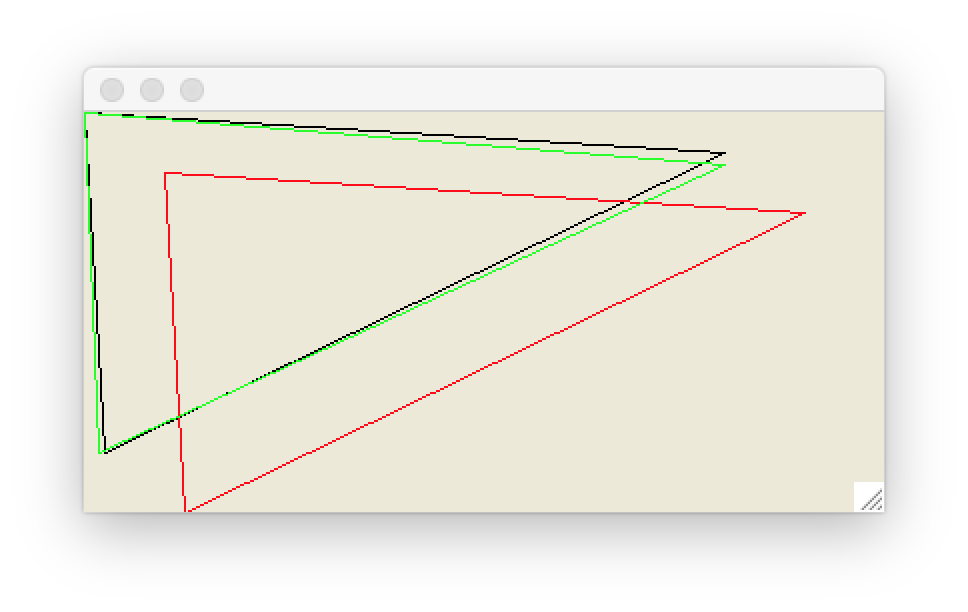
\includegraphics[width=0.6\textwidth]{transformWindows}
  \caption{Transformed versions of the same triangle resulting from running the code in Listing~\ref{winforms/transformWindows}.}
  \label{fig:transformWindow}
\end{figure}
We now have a basis for solving the following problem:
\begin{problem}
  Given a triangle produce a Mandela drawing, where $n$ rotated versions of the triangle is drawn around its center of mass.
\end{problem}
Reusing the top part of Listing~\ref{winforms/transformWindows} and replacing the bottom part with the code shown in Listing~\ref{winforms/rotationalSymmetry}, we arrive a the solution illustrated in Figure~\ref{fig:rotationalSymmetry}.
%
\fsCode[numbers=left,numbersep=6pt,numberstyle=\scriptsize\color{white},firstnumber=44,firstline=44]{winforms/rotationalSymmetry}{Create the window and changing its properties.}
%
\begin{figure}
  \centering
  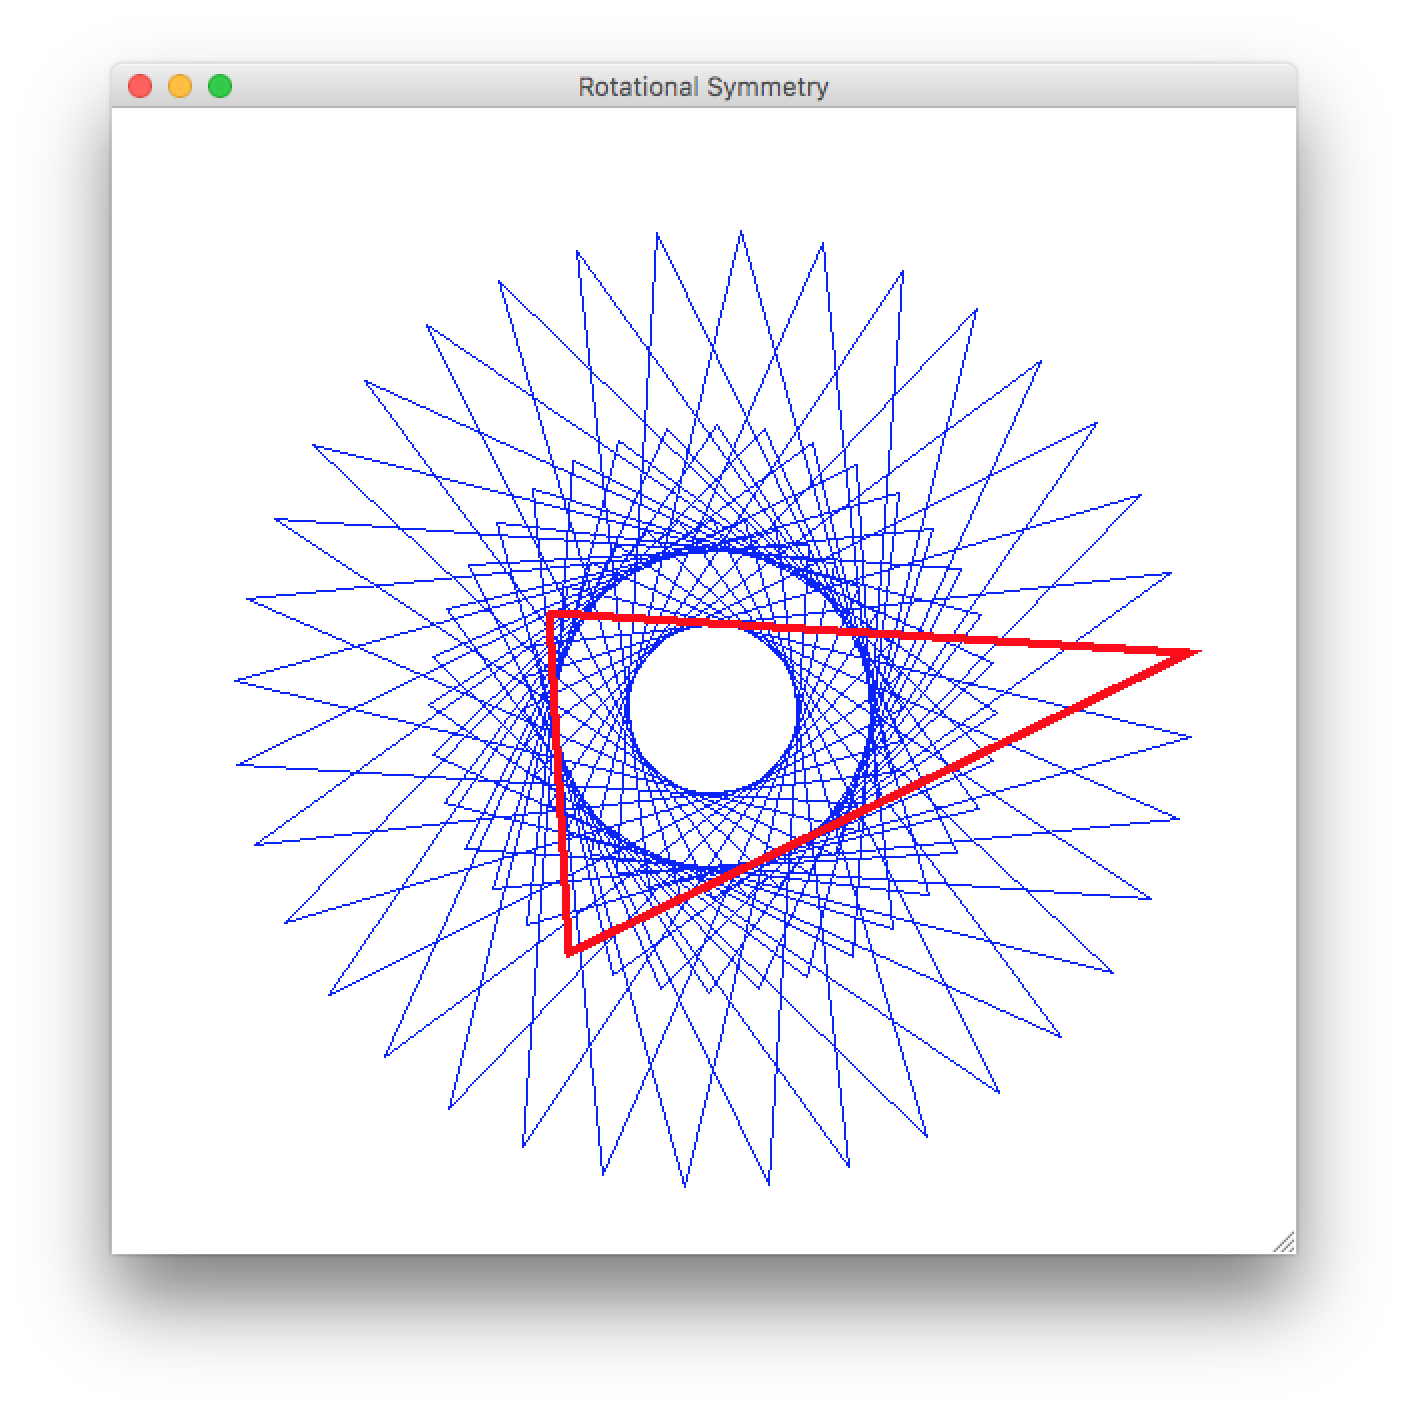
\includegraphics[width=0.8\textwidth]{rotationalSymmetry}
  \caption{A symmetric figure resulting from Listing~\ref{winforms/rotationalSymmetry}.}
  \label{fig:rotationalSymmetry}
\end{figure}
\jon{Remember to add something on piping.}

The \lstinline!System.Drawing.Graphics! class contains many other algorithms for drawing graphics primitives, some of which are listing in Table~\ref{tab:graphicsMethods}
\begin{table}
  \begin{center}
  \rowcolors{2}{oddRowColor}{evenRowColor}
    \begin{tabularx}{\linewidth}{|l|X|}
      \hline
      \rowcolor{headerRowColor}  Function & Description\\
      \hline
      \lstinline{DrawArc : Pen * Rectangle * Single * Single}
      &Draws an arc representing a portion of an ellipse specified by a Rectangle structure.\\
      \hline
      \lstinline{DrawBezier : Pen * Point * Point * Point * Point}	
      &Draws a Bézier spline defined by four Point structures.\\
      \hline
      \lstinline{DrawCurve : Pen * Point[]}	
      &Draws a cardinal spline through a specified array of Point structures.\\
      \hline
      \lstinline{DrawEllipse : Pen * Rectangle}	
      &Draws an ellipse specified by a bounding Rectangle structure.\\
      \hline
      \lstinline{DrawImage : Image * Point[]}	
      &Draws the specified Image at the specified location and with the specified shape and size.\\
      \hline
      \lstinline{DrawLine : Pen * Point * Point}	
      &Draws a series of line segments that connect an array of Point structures.\\
      \hline
      \lstinline{DrawLines : Pen * Point[]}	
      &Draws a series of line segments that connect an array of Point structures.\\
      \hline
      \lstinline{DrawPie : Pen * Rectangle * Single * Single}	
      &Draws a pie shape defined by an ellipse specified by a Rectangle structure and two radial lines.\\
      \hline
      \lstinline{DrawPolygon : Pen * Point[]}	
      &Draws a polygon defined by an array of Point structures.\\
      \hline
      \lstinline{DrawRectangles : Pen * Rectangle[]}	
      &Draws a series of rectangles specified by Rectangle structures.\\
      \hline
      \lstinline{DrawString : String * Font * Brush * PointF}	
      &Draws the specified text string at the specified location with the specified Brush and Font objects.\\
      \hline
      \lstinline{FillClosedCurve : Brush * Point[]}	
      &Fills the interior of a closed cardinal spline curve defined by an array of Point structures.\\
      \hline
      \lstinline{FillEllipse : Brush * Rectangle}	
      &Fills the interior of an ellipse defined by a bounding rectangle specified by a Rectangle structure.\\
      \hline
      \lstinline{FillPie : Brush * Rectangle * Single * Single}	
      &Fills the interior of a pie section defined by an ellipse specified by a RectangleF structure and two radial lines.\\
      \hline
      \lstinline{FillPolygon : Brush * Point[]}	
      &Fills the interior of a polygon defined by an array of points specified by Point structures.\\
      \hline
      \lstinline{FillRectangle : Brush * Rectangle}	
      &Fills the interior of a rectangle specified by a Rectangle structure.\\
      \hline
    \end{tabularx}
  \end{center}
  \caption{Some methods of the \lstinline!System.Drawing.Graphics! class.}
  \label{tab:graphicsMethods}
\end{table}
\jon{Give examples of more methods}

\section{Programming intermezzo}
Reusing the top part of Listing~\ref{winforms/transformWindows} we are now able to tackle complicated problems such as space-filling curves. A curve in 2 dimensions has a length but no width, and we can only visualize it by giving it a width. It is thus came as a surprise to many when Giuseppe Peano in 1890 demonstrated that there exists curves, which fill every point in a square. The method he used to achieve this was recursion.
\begin{problem}
  Consider a curve consisting of piecewise straight lines all with the same length but with varying angles $0^{\circ}$, $90^{\circ}$, $180^{\circ}$, or $270^{\circ}$ w.r.t.\ the horisontal axis. To draw this curve we need 3 basic operations: Move forward ($F$), turn right ($+$), and turn left ($-$). The turning is w.r.t.\ the present direction. A Hilbert Curve is a space-filling curve, which be expressed recursively as:
\begin{align}
  A &\rightarrow -BF+AFA+FB-\label{eq:hilbertA}\\
  B &\rightarrow +AF-BFB-FA+\label{eq:hilbertB}
\end{align}
starting with $A$. For practical illustrations, we typically only draw space filling curves to a specified depth of recursion, which is called the order of the curve. Hence, to draw a first order curve, we don't recurse at all, i.e., ignore all occurrences of the symbols $A$ and $B$ on the right-hand-side of \eqref{eq:hilbertA}, and get 
\begin{align*}
  A \rightarrow -F+F+F-. 
\end{align*}
For the second order curve, we recurse once, i.e., 
\begin{align*}
  A 
  \rightarrow &-BF+AFA+FB- \\
  \rightarrow &-(+AF-BFB-FA+)F\\
               &\quad+(-BF+AFA+FB-)F(-BF+AFA+FB-)\\
               &\qquad +F(+AF-BFB-FA+)-\\
  \rightarrow &AF-BFB-FA+FBF+AFA+FB-F-BF+AFA+FBF+AF-BFB-FA\\
  \rightarrow &F-F-F+FF+F+F-F-F+F+FF+F-F-F.
\end{align*}
Make a program, that given an order produces an image of the Hilbert curve.
\end{problem}
Our strategy will be to draw the curve sequentially from the origin to the end point. For this we will make a data structure \lstinline!type curve = float * float * coordinates)! length and the orientation of the next forward move and a partial list straight line pieces. The initial point would thus be \lstinline(1.0, 0.0, [(0.0, 0.0)]). We will also make 2 mutually recursive functions \lstinline!ruleA : float curve -> curve! and \lstinline!ruleB : float curve -> curve!, which takes n order and our data structure as input and for positive orders adds its rule to the end of the curve. We also need the three basic operations. To move forward, we will use the \lstinline!rotatePoint! and \lstinline!translatePoint! functions from Listing~\ref{winforms/transformWindows}, that is, we may take line piece of specified length starting in the origin, rotate it according to the present orientation of the curve, and translate it to the present end-point of the curve. The two turn right and left only need to add or subtract $90^{\circ}$ to the present orientation. Thus, reusing the top part of Listing~\ref{winforms/transformWindows} we arrive at the solutions shown in Listing~\ref{winforms/hilbert}. In Figure~\ref{fig:hilbert} are shown the result of using the program to draw Hilbert curves of orders 1, 2, 3, and 5.
%
\fsCode[numbers=left,numbersep=6pt,numberstyle=\scriptsize\color{white},firstnumber=44,firstline=44]{winforms/hilbert}{Create the window and changing its properties.}
%
\begin{figure}
  \centering
  \subfigure[Order 1]{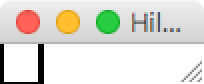
\includegraphics[scale=0.25]{hilbert1}}
  \subfigure[Order 2]{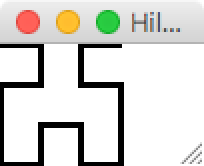
\includegraphics[scale=0.25]{hilbert2}}
  \subfigure[Order 3]{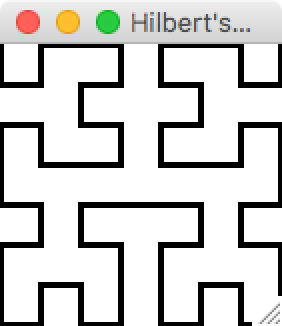
\includegraphics[scale=0.25]{hilbert3}}
  \subfigure[Order 5]{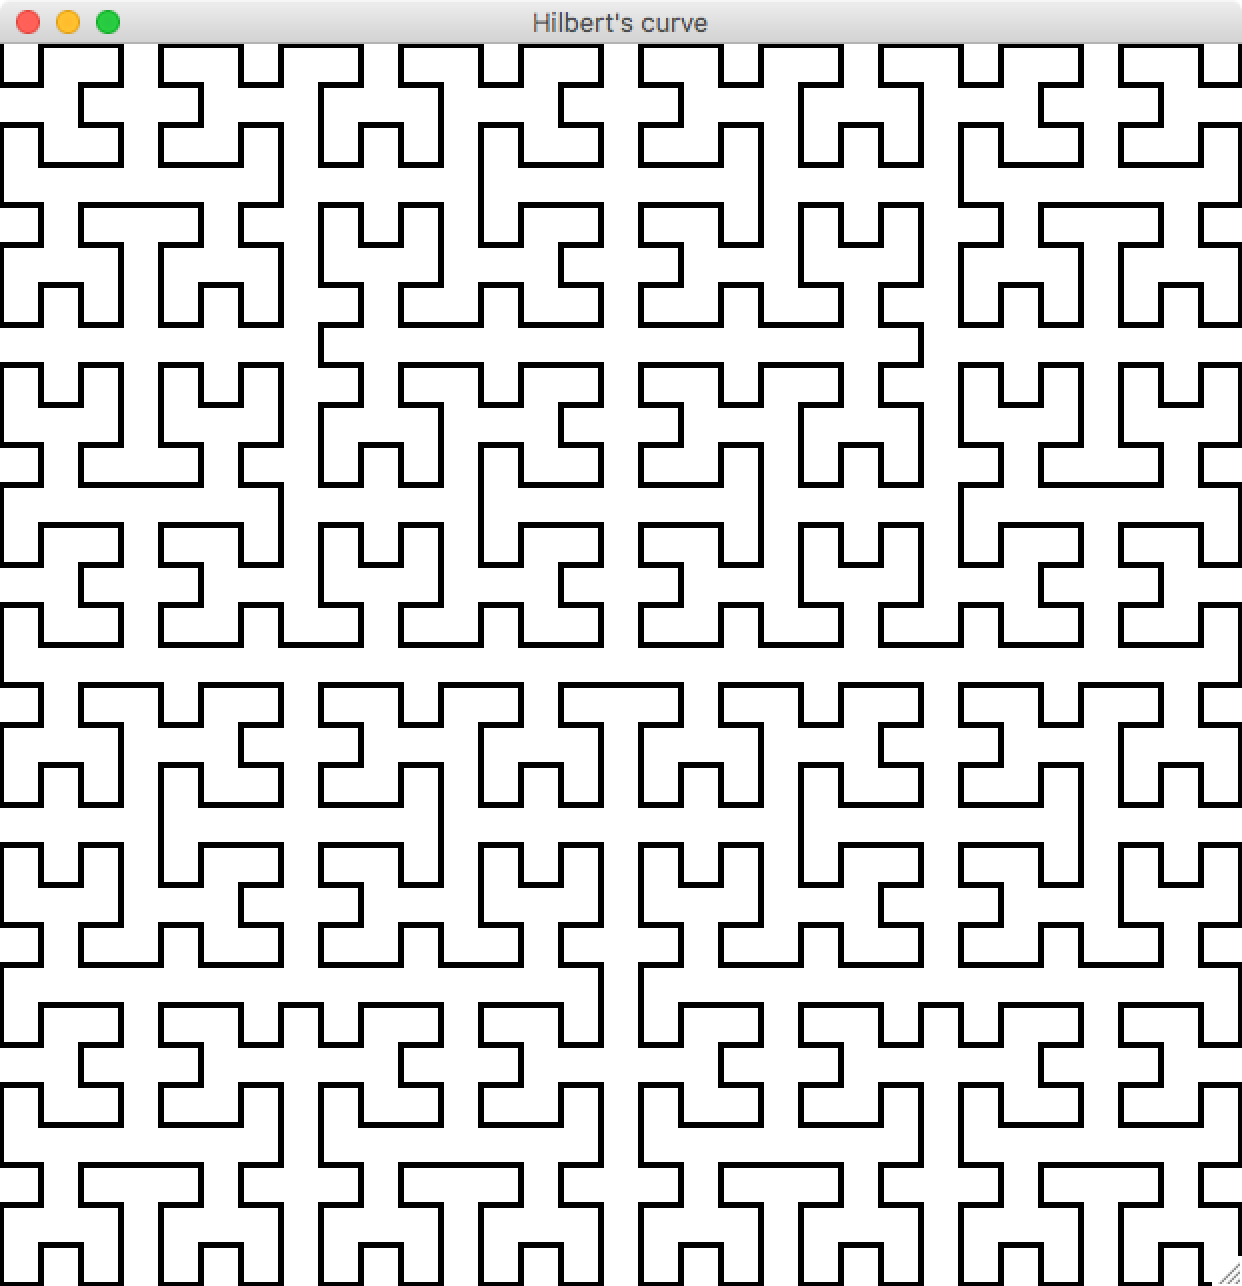
\includegraphics[scale=0.25]{hilbert5}}
  \caption{Hilbert curves of order 1, 2, 3, and 5 by code in Listing~\ref{winforms/hilbert}.}
  \label{fig:hilbert}
\end{figure}

\section{Events, Controls, and Panels}
In the previous section, we have looked at how to draw graphics using the \lstinline!Paint! method of an existing form object. Forms have many other event listeners, that we may use to interact with the user. Listing~\ref{winforms/windowEvents} demonstrates event handlers for moving and resizing a window, for clicking in a window, and for typing on the keyboard.
%
\fsCode{winforms/windowEvents}{Catching window, mouse, and keyboard events.}
%
\fsOutput{winforms/windowEvents}{Output from an interaction with the program in Listing~\ref{winforms/windowEvents}.}
%
In Listing~\ref{winforms/windowEvents} is shown the output from an interaction with the program which is the result of the following actions: moving the window, resizing the window, clicking the left mouse key, pressing and holding the down the left mouse key while moving the mouse, and releasing the left mouse key, and type ``fsharp''. As demonstrated, some actions like moving the mouse results in a lot of events, and some like the initial window moves results are surprising. Thus, event drivent programming should take care to interpret the events robustly and carefully.

In WinForms buttons, menus and other interactive elements are called \idx{Controls}. A form is a type of control, and thus, programming controls are very similar to programming windows. In Listing~\ref{winforms/buttonControl} is shown a small program that displays a button in a window, and when the button is pressed, then a dialogue is opened in another window. Figure~\ref{fig:buttonControl} shows an example dialogue.
%
\fsCode{winforms/buttonControl}{Create the button and an event.}
%
\begin{figure}
  \centering
  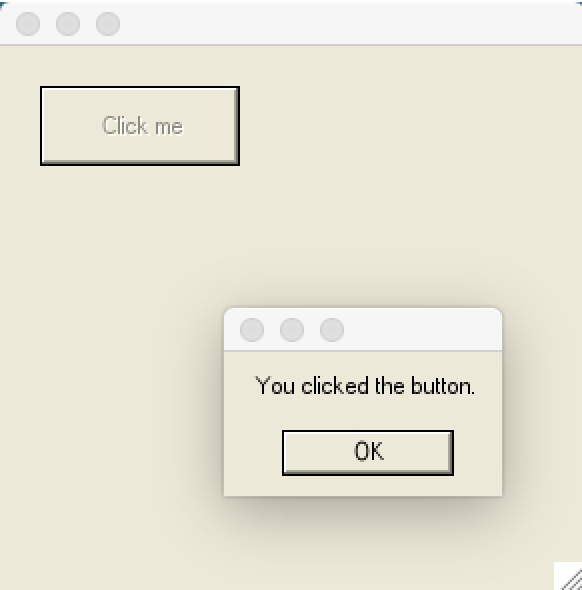
\includegraphics[width=0.6\textwidth]{buttonControl}
  \caption{A button is pressed and the event handler calls the \lstinline!MessageBox.Show! dialogue window by the code in Listing~\ref{winforms/buttonControl}.}
  \label{fig:buttonControl}
\end{figure}
%
As the listing demonstrates, the button is created using the \idx{\lstinline{System.Windows.Forms.Button}} constructor, and it is added to the form's control list. It is possible to have many controls on each form, but at times it is useful to organize the controls in groups. Such groups are called \idx{Panels} in WinForms, and an example of creating a \idx{\lstinline{System.Windows.Forms.Panel}} that includes a \idx{\lstinline{System.Windows.Forms.TextBox}} and \idx{\lstinline{System.Windows.Forms.Label}} for getting user input is shown in Listing~\ref{winforms/panel} and Figure~\ref{fig:panel}. 
%
\fsCode{winforms/panel}{Create a panel, label, text input controls.}
%
\begin{figure}
  \centering
  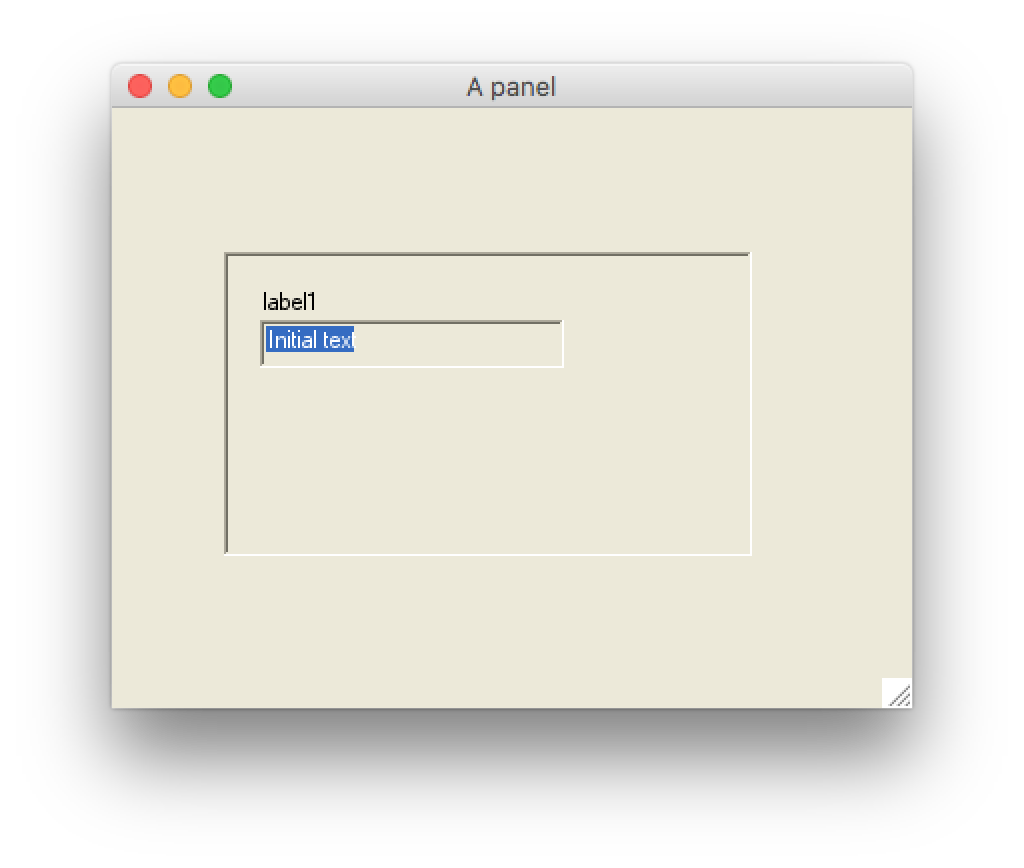
\includegraphics[width=0.6\textwidth]{panel}
  \caption{A panel including a label and a text input field, see Listing~\ref{winforms/panel}.}
  \label{fig:panel}
\end{figure}
The label and textbox are children of the panel, and the main advantage of using panels is that the coordinates of the children are relative to the top left corner of the panel. I.e., moving the panel will move the label and the textbox at the same time.

Several types of panels exists in WinForms. A very flexible panel is the \idx{\lstinline{System.Windows.Forms.FlowLayoutPanel}}, which arranges its objects according to the space available. This is useful for graphical user interfaces targeting varying device sizes, such as a computer monitor and a tablet, and it also allows the program to gracefully adapt, when the user changes window size. A demonstration of \lstinline{System.Windows.Forms.FlowLayoutPanel} together with \lstinline{System.Windows.Forms.CheckBox} and \lstinline{System.Windows.Forms.RadioButton} is given in Listing~\ref{winforms/flowLayoutPanel} and in Figure~\ref{fig:flowLayoutPanel}. The program illustrates how the button elements flow under four possible \lstinline{System.Windows.FlowDirection}s, and how \lstinline{System.Windows.WrapContents} influences, what happens to content that flows outside the panels region. 
%
\fsCode[lastline=34]{winforms/flowLayoutPanel}{Create a FlowLayoutPanel, with checkbox and radiobuttons.}
%
%
\fsCode[firstline=36,firstnumber=36]{winforms/flowLayoutPanel}{Create a FlowLayoutPanel, with checkbox and radiobuttons.}
%
\begin{figure}
  \centering
  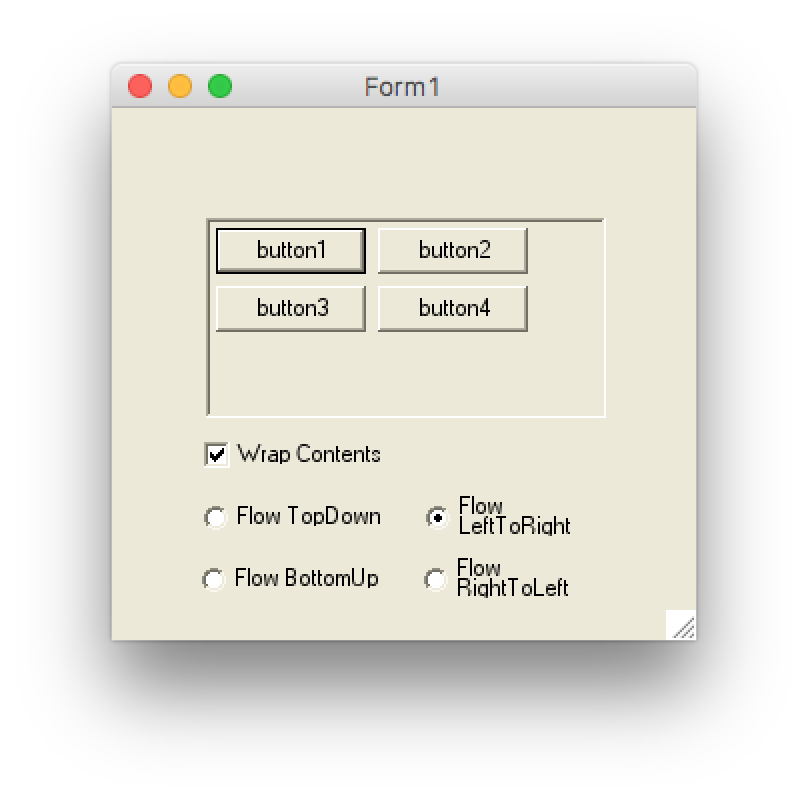
\includegraphics[width=0.6\textwidth]{flowLayoutPanel}
  \caption{Demonstration of the \lstinline!FlowLayoutPanel! panel, \lstinline!CheckBox!, and \lstinline!RadioButton! controls, see Listing~\ref{winforms/flowLayoutPanel}.}
  \label{fig:flowLayoutPanel}
\end{figure}
A walkthrough of the program is as follows. The goal is to make 2 areas, one giving the user control over display parameters, and another displaying the result of the user's choices. These are \lstinline{FlowLayoutPanel} and \lstinline{Panel}. In the \lstinline{FloatLayoutPanel} there are four \lstinline{Button}s, to be displayed in a region, that is not tall enough for the buttons to be shown in vertical sequence and not wide enough to be shown in horizontal sequence. Thus the \lstinline{FlowDirection} rules come into play, i.e., the buttons are added in sequence as they are named, and the default \lstinline{FlowDirection.LeftToRight} arranges places the \lstinline{buttonLst.[0]} in the top left corner, and \lstinline{buttonLst.[1]} to its right. Other flow directions does it differently, and the reader is encourage to experiment with the program.

The program in Listing~\ref{winforms/flowLayoutPanel} has not completely separated the semantic blocks of the interface and relies on explicitly setting of coordinates of controls. This can be avoided by using nested panels. E.g., in Listing~\ref{winforms/flowLayoutPanelAdvanced}, the program has been rewritten as a nested set of \lstinline{FloatLayoutPanel} in three groups: The button panel, the checkbox, and the radio button panel. Adding a \lstinline{Resize} event handler for the window to resize the outermost panel according to the outer window, allows for the three groups to change position relative to each other, which results in three different views all shown in Figure~\ref{fig:flowLayoutPanelAdvanced}.
%
\fsCode[lastline=42]{winforms/flowLayoutPanelAdvanced}{Create nested FlowLayoutPanel.}
%
%
\fsCode[firstline=44,firstnumber=44]{winforms/flowLayoutPanelAdvanced}{Create nested FlowLayoutPanel, see Listing~\ref{winforms/flowLayoutPanelAdvanced}.}
%
\begin{figure}
  \centering
  \subfigure[]{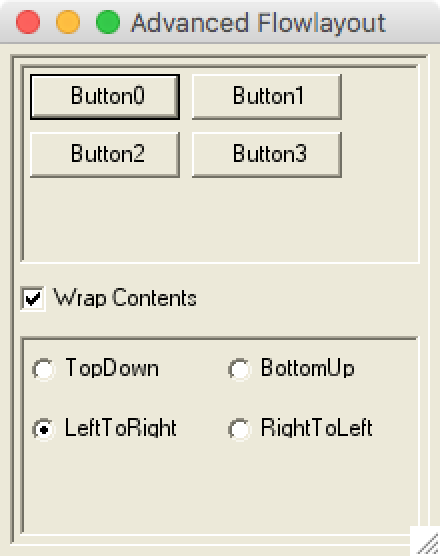
\includegraphics[width=0.3\textwidth]{flowLayoutPanelAdvanced}}
  \subfigure[]{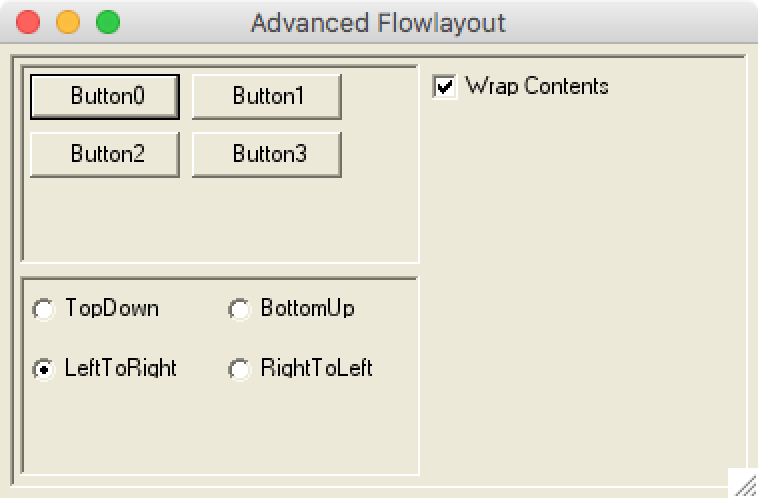
\includegraphics[width=0.6\textwidth]{flowLayoutPanelAdvanced2}}
  \subfigure[]{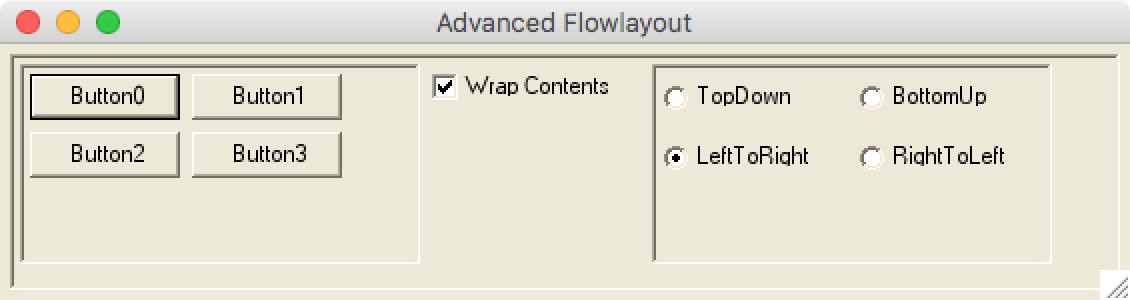
\includegraphics[width=0.9\textwidth]{flowLayoutPanelAdvanced3}}
  \caption{Nested \lstinline!FlowLayoutPanel!, see Listing~\ref{winforms/flowLayoutPanelAdvanced}, allows for dynamic arrangement of content. Content flows, when the window is resized.}
  \label{fig:flowLayoutPanelAdvanced}
\end{figure}
\jon{Add simple panel code \lstinline!simpleFlowLayoutPanel.fsx! and \lstinline!simpleTableLayoutPanel.fsx!.}  
\jon{Add \lstinline{Dock}, \lstinline{Padding} structure, \lstinline{Margin}, \lstinline{Padding}, \lstinline{Controls.AddRange} , and \lstinline{AutoSize} properties. Add figure, e.g., \lstinline!IC138411.jpeg.gif!.}
\jon{Add \lstinline{GroupBox} and discuss difference to \lstinline{Panel}.}

%
\fsCode{winforms/simpleFlowLayoutPanel}{\dots}
%
\begin{figure}
  \centering
  \subfigure[]{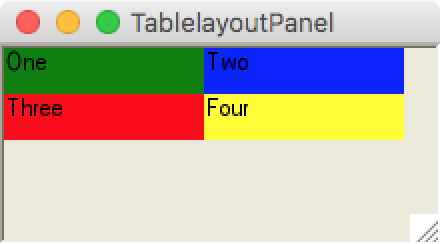
\includegraphics[width=0.45\textwidth]{simpleFlowLayoutPanel1}}
  \subfigure[]{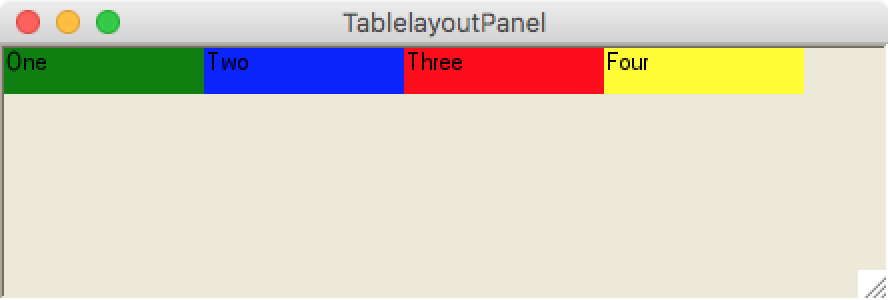
\includegraphics[width=0.9\textwidth]{simpleFlowLayoutPanel2}}
  \subfigure[]{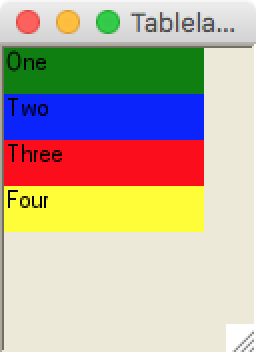
\includegraphics[width=0.225\textwidth]{simpleFlowLayoutPanel3}}
  \caption{See Listing~\ref{winforms/simpleFlowLayoutPanel}.}
  \label{fig: simpleFlowLayoutPanel}
\end{figure}

%
\fsCode{winforms/simpleTableLayoutPanel}{\dots}
%
\begin{figure}
  \centering
  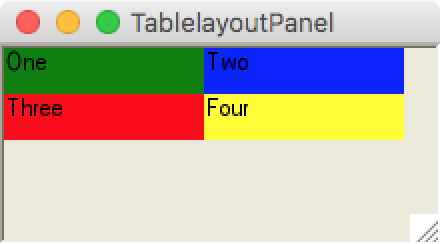
\includegraphics[width=0.4\textwidth]{simpleTableLayoutPanel}
  \caption{See Listing~\ref{winforms/simpleTableLayoutPanel}.}
  \label{fig: simpleTableLayoutPanel}
\end{figure}

%
\fsCode{winforms/bounds}{\dots}
%
\begin{figure}
  \centering
  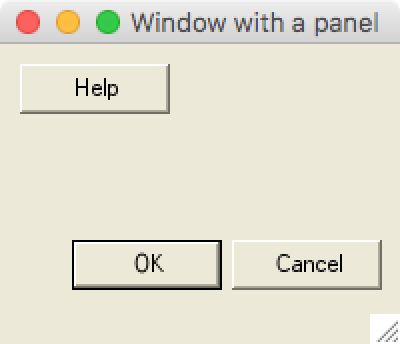
\includegraphics[width=0.3\textwidth]{bounds}
  \caption{See Listing~\ref{winforms/bounds}.}
  \label{fig:bounds}
\end{figure}

%
\fsCode{winforms/tabControl}{\dots}
%
\begin{figure}
  \centering
  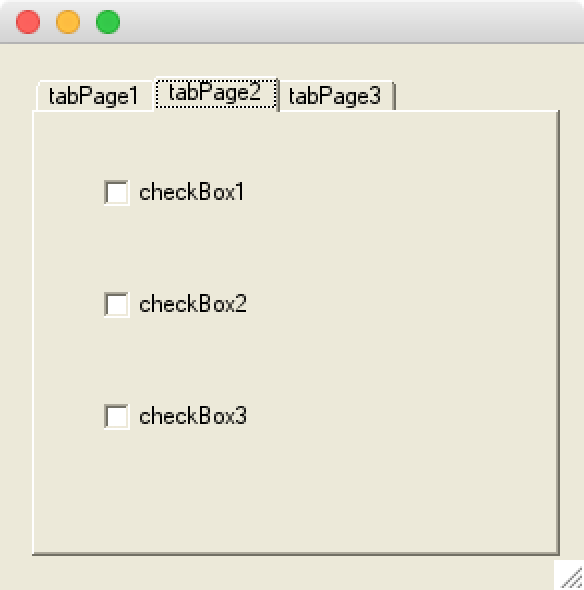
\includegraphics[width=0.3\textwidth]{tabControl}
  \caption{See Listing~\ref{winforms/tabControl}.}
  \label{fig: tabControl}
\end{figure}

%
\fsCode{winforms/trackBar}{\dots}
%
\begin{figure}
  \centering
  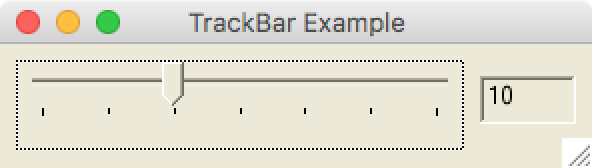
\includegraphics[width=0.3\textwidth]{trackBar}
  \caption{See Listing~\ref{winforms/trackBar}.}
  \label{fig: trackBar}
\end{figure}

%
\fsCode{winforms/progressBar}{\dots}
%
\begin{figure}
  \centering
  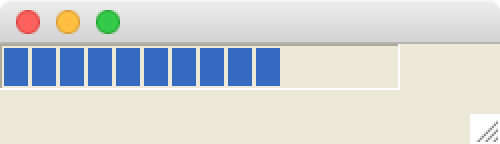
\includegraphics[width=0.3\textwidth]{progressBar}
  \caption{See Listing~\ref{winforms/progressBar}.}
  \label{fig:bounds}
\end{figure}

%%% Local Variables:
%%% TeX-master: "fsharpNotes"
%%% End:
